\section{A Single Promoter Inversion Switches Photorhabdus Between Pathogenic and Mutualistic States}

\subsection{Нормальное название}

Одна инверсия промотора приводит к переключении бактерии Photorhabdus между патогенным и мутуалистическим состоянием.
\subsection{Абстракт}
Популяции микробов случайным образом генерируют варианты с совершенно разными свойствами, такими как вирулентность(способность вызывать заболевания) или авирулентность, толерантность (чувствительность) к антибиотикам. Бактерии Photorhabdus luminescens имеют разнообразную жизненную историю, в которой они чередуются между патогенами к множеству насекомых и мутуалистами с их нематодами-хозяевами. В статье мы показываем, что патогенный вариант P. luminescens (форма P) переключается на вариант с меньшими (по размеру) клетками (форма M), чтобы инициировать мутуализм в кишечнике немато-хозяев (они в них живут). Стохастическая инверсия промотора вызывает переключение между двумя различными формами. Клетки M-формы намного меньше (одна седьмая объема), медленнее растут и менее биолюминесцентны, чем клетки P-формы; они также авирулентны и производят меньше вторичных метаболитов (продукты метаболизма, которые НЕ необходимы для жизни). Наблюдения за переключением формы отдельными клетками в нематодах показали, что форма М сохранялась в кишечнике материнской нематоды, и была первыми клетками, колонизировавшими инфекционное молодое (IJ - infective juvenile) потомство (нематод), а затем переключилась на P-форму в кишечнике IJ, которая дала возможность нематодам заражать следующий цикл насекомых.


\subsection{Картинки}
\begin{figure}[H]\label{ul}
	\center{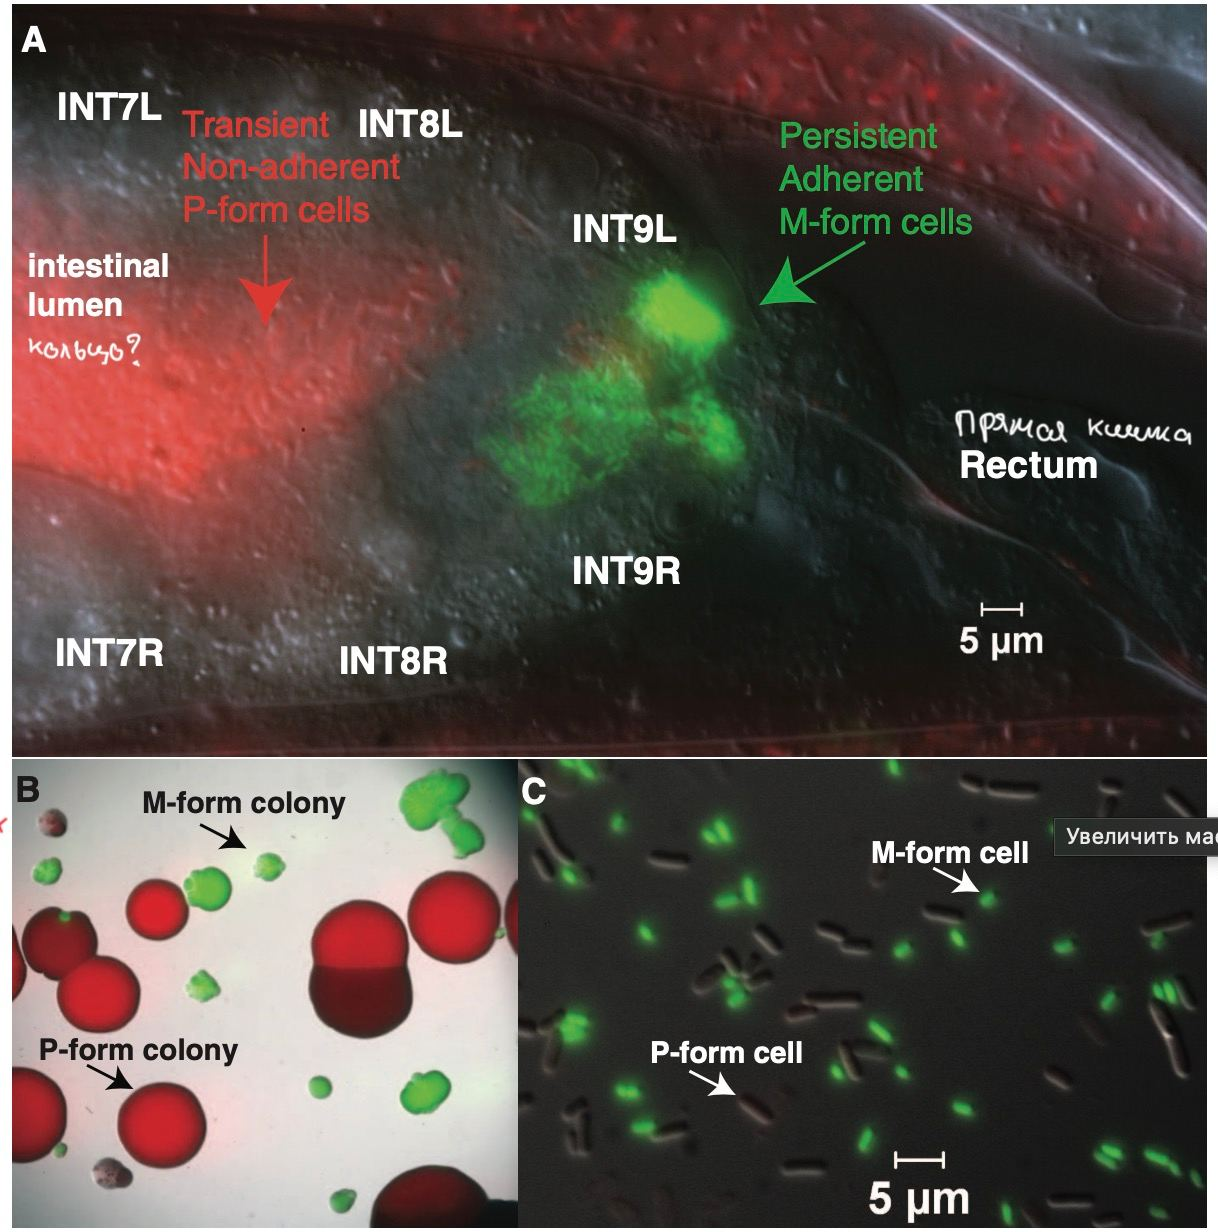
\includegraphics[scale=0.3]{a31.jpg}}
	\caption{Первая картинка}
\end{figure} 


Значит на первой пикче \textbf{(а)}
Дело происходит в кишечнике нематоды (глисты). Все эти инты — номера колец в кишечнике, типа геотег
Зелёные — М-форма этих бактерий, она меньше и устойчива (в плане статична, так как они отвечают непосредственно за прилипание (по-умному адгезия)). Красные — П-форма — отвечают за заразность по отношению к насекомым, в которых селятся их нематоды (в кишечнике которых они находятся), территориально они находятся в люмене (внутренне пространство в кишечнике этой ебаной нематоды).



\textbf{Пикча б)}
Нарисованы КОЛОНИИ, а не сами бактерии. Пишут, что красные (П-форму) образуют большие колонии, а зелёные (М-форма) маленькие (вау, охуеть, да?). 

\textbf{Пикча ц)}
Нарисованы сами бактерии, их характерный размер. Пишут примерно то же самое. Зелёные — бактерии М-формы, красные — П-формы (которая больше по размерам, чем М-форма).


\begin{figure}[H]\label{ul}
	\center{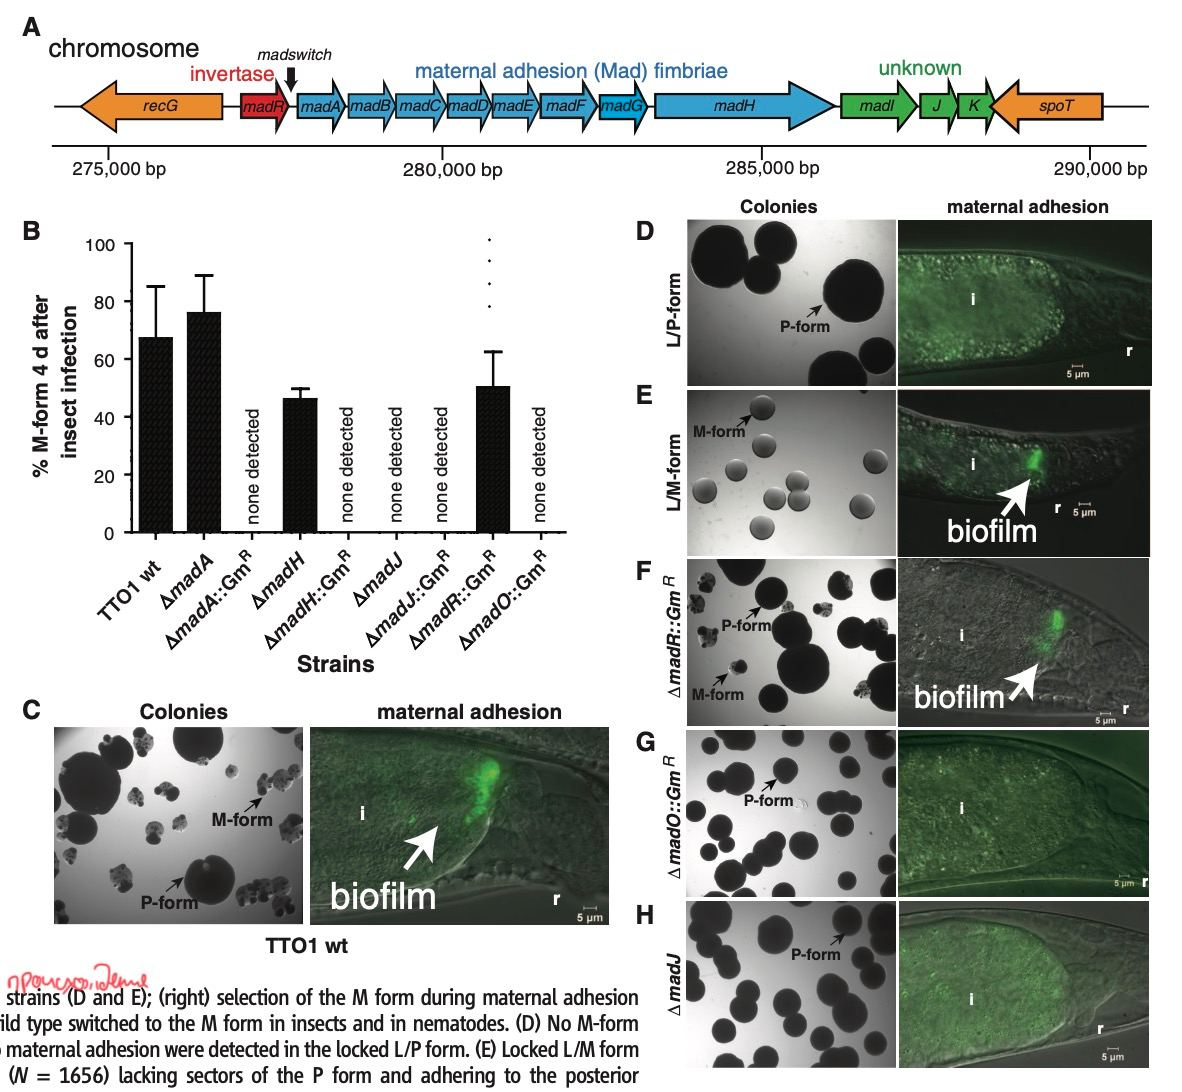
\includegraphics[scale=0.3]{a32.jpg}}
	\caption{Вторая картинка}
\end{figure} 

\textbf{Картинка а)}
Нарисована хромосома (ФЕЗЕЧЕСКАЯ КАРТА)
Все эти  mad..  — гены. Мадсвитч — как раз тот самый участок-промотор (участок хромосомы, инициирующий трансляцию). БП — пары нуклеотдиов, в них всё измеряется
МадР (инвертаза, то есть отвечаает за инверсию) — нихуя не меняет, избыточен для того, чтобы включать инверсию. Дальше про гены нигде не написано, про которую нигде не написано. Стрелка — направление транскрипции (считывания)
\\
\\
\textbf{б — гистограмма говна}. По вертикальной оси процент бактерий в М-форме от всей колонии через 4 дня после инфецирования насекомого (П-формой). Усы — стандартное отклонения
Дельта — делеция (удаление нахуй примерно), ::Gm добавление на это место какой-то хуеты. 
По иксам — TT01 — дикая форма, в которую ничего не добавляли (П-форма).  Думаю, что подписывать процентики это всратоо. Ноне детектион — не нашли М-форму вообще
\\
\\
\textbf{ц-х} — Обозначения — аналогичные. Слева нарисованы колонии, справа кишка нематоды. И — кишечник, р — ректум (жепа). Биофилм — множество микроорганизмов, расположенных на какой-либо поверхности, клетки которых прикреплены друг к другу. L/…-form — заблокирован определённый ген, который отвечает за этот свитч как раз. То есть бактерия по сути застряла в одной форме.

Гляди на картинке, наличие биоплёнки или ярко-зелёного цвета говорит тебе о том, что появились М-форма. Достаточно в принципе посмотреть на колонии. 

В случае пикчи аш надо сказать, что в 54 процентах исследованых нематод не было прикреплённый (адгезированных) бактерий

\begin{figure}[H]\label{ul}
	\center{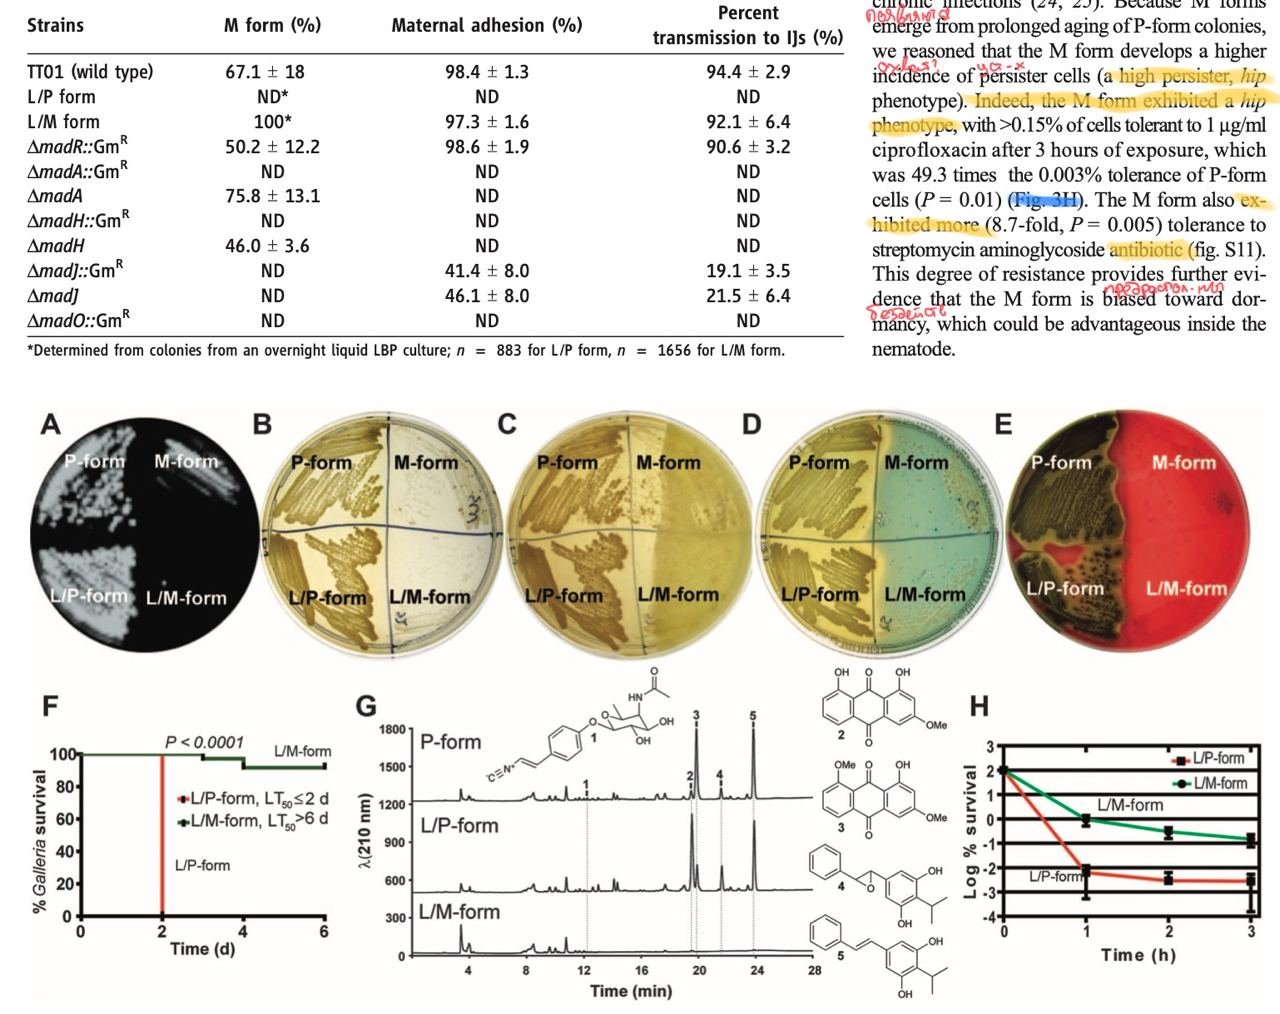
\includegraphics[scale=0.3]{a33.jpg}}
	\caption{Третья картинка}
\end{figure} 
\textbf{Табличка — первая колонка} — типы введённых клеток, вторая — М-форма клеток в насекомых через 4 дня после того, как вводили П-форму, третья — процент адгезировавших(??) бактерий в кишечнике материнской нематоды через 38-40 часов (в 40-60 нематодах). Четвёртая — передача в заразное потомство (возрастом в 7 дней). +- — Стандартное отклонение
\\
\\
\textbf{А,Б,Ц,Д,Е} — чашка петри разделена на 4 части. Лево верх — простая п-форма, право верх — простая М-форма, лево низ — «фиксированная» (вмороженная) П-форма, право низ — «фиксированная» (вмороженная) М-форма
\\
\\
\textbf{А} — Свечение, которое производят соответствующие бактерии (отмечают, что в М-форме светятся мутанты, которые частично приобретают свойства П-формы)
\textbf{Б} — Сравнивают цвет, П-форма непрозрачная и жёлтая, М-форма прозрачная и непигментированная (всм бесцветная)
\textbf{Ц} — Антимикробная активность за 48 часов роста на LBP (lysogeny broth plus sodium pyruvate) по отношению к бактерии Micrococcus luteus
\textbf{Д} — Насколько активно происходило хелатирование (расщепление) железа. Для П-формы активно, для М-формы нет. Зона очищается по мере того, как железо расщепляется. 
\textbf{Е} — Насколько активно разрушают красные кровяные тельца на примере крови овцы. П-форма активно, М-форма вообще не разрушает
\\
\\
\textbf{Ф} — Вирулентность (способность производить вредные вещества) М-формой и П-формой для насекомых Galleria mellonella(личинок). (LT50 — время, когда умирало 50 процоентов исследуемых особей)
\\
\\
\textbf{Ж} — Метаболитный анализ показал, что бактерии могут вырабатывать rhabduscin (химическая формула 1, под ней есть на число на графике, я так понял, что это момент его производства). Далее аналогично 2,3 — антрахинонные пигментные молекулы (которые и дают жёлтый цвет). 4,5 — гидроксистильбеновые молекулы, котоорых практически нет в вмороженной М-форме. 
\\
\\
\textbf{Аш} — График логарифма процента выживших от времени после введения 1 мкг/мл ciprofloxacin (антибиотик) за три часа наблюдений (Вмороженная М-форма форма в 50 раз более устойчивая к антибиотикам)

\begin{figure}[H]\label{ul}
	\center{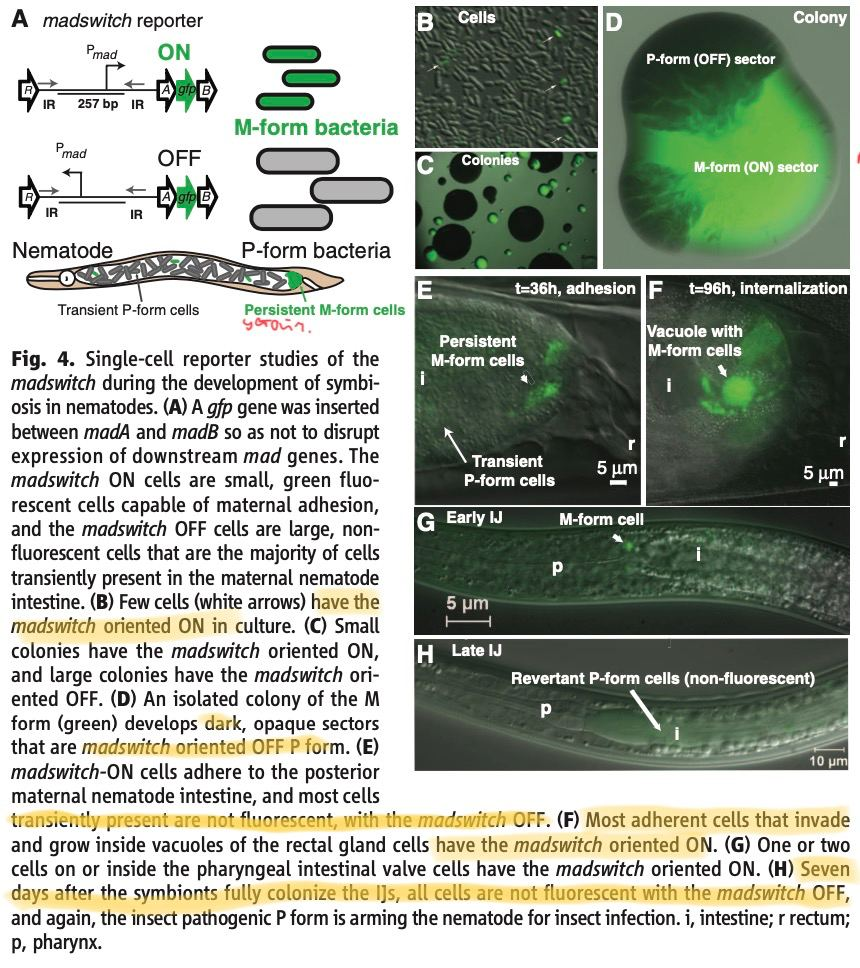
\includegraphics[scale=0.3]{a34.jpg}}
	\caption{Четвертая  картинка}
\end{figure} 

\textbf{А} — о том, как красили М-форму. Так как форма связана с направлением проомотора, то они добавляли красящий ген после проомотора (через 1 ген, чтобы не влиять на остальные гены).
У клеток с направлением промотора  ON клетки маленькие и светятся зелёным, способные к адгезии. С направлением промотороа OFF — клетки большие, не светятся, котороые не прикрепляются ни к чему в кишечнике материнской нематоды. Внизу картинки А изображено местоположение клеток в нематоде (серые — «плавающая» по кишечнику П-форма, зелёные — прикреплённая М-форма)
\\
\\
\textbf{Б} — у некоторых бактерий в культуре проомотор (madswitch) ориентрован ONю Эти бактерии зелёные, на них указывает стрелка
\\
\\
\textbf{Ц} — маленькие колонии имеют madswitch с ориентацией ON (зелёные, M-форма). Большие колонии имеют madswitch с ориентацией OFF (чёрные, П-форма)
\\
\\
\textbf{D} — В изолированной колонии бактерий ON появляются тёмные непрозрачные участки бактерий OFF
\\
\\
\textbf{E} —Показывают, что ON бактерии прикрепляются к кишечнику нематоды, а большинство ‘плавающих’ — не светятся, то есть OFF-бактерии. 
\\
\\
\textbf{F} — Большинство прикреплённых клеток, которые прикрепляются к rectal gland и растут внутри клеток вакуолей этой rectal gland это ON-бактерии
\\
\\
\textbf{G} - В раннем заразном потомсвте несколько клеток бактерий в кишечнике имеют madswitch направленный ON.
\\
\\
\textbf{H} — Через неделю после того, как симбиоты полностью колонизируют заразное потомство клетки перестают светиться, а значит, что развились мутанты с направлением OFF. То есть по сути в конце внутри нематоды остаётся только патогенная форма, которая нужна нематодам для заражения насекомых

На картинках i — кишечник p — глотка, r — прямая кишка